\documentclass[12pt,english,a4paper]{article}
\pdfobjcompresslevel=0
\usepackage[usenames,dvipsnames]{xcolor}
\usepackage[includeheadfoot,margin=0.8 in,top=0.6 in]{geometry}
\usepackage{siunitx,physics,cancel,upgreek,varioref,listings,booktabs,tocloft, pdfpages}
\usepackage{mathtools}
\usepackage{babel}
\usepackage{graphicx}
\usepackage{float}
\usepackage{fouriernc}
\usepackage{fancyhdr}
\usepackage[utf8]{inputenc}
\usepackage{amsmath}
\usepackage{amssymb}
\usepackage{textcomp}
\usepackage{lastpage}
\usepackage{microtype}
\usepackage{ifthen}
\usepackage{longtable}
\usepackage[linktoc=all, bookmarks=true, pdfauthor={Anders Johansson}]{hyperref}
\renewcommand{\CancelColor}{\color{red}}
\renewcommand{\exp}[1]{\mathrm{e}^{#1}}
\newcommand{\R}{\mathbb{R}}
\newcommand{\tittel}[1]{\title{#1 \vspace{-7ex}}\author{}\date{}\maketitle\thispagestyle{fancy}\pagestyle{fancy}\setcounter{page}{1}}

\newcommand{\deloppg}[2][]{\subsection*{#2) #1}\addcontentsline{toc}{subsection}{#2)}\refstepcounter{subsection}\label{#2}}
\newcommand{\oppg}[1]{\section*{Oppgave #1}\addcontentsline{toc}{section}{Oppgave #1}\refstepcounter{section}\label{oppg#1}}

\labelformat{section}{section~#1}
\labelformat{subsection}{section~#1}
\labelformat{subsubsection}{paragraph~#1}
\labelformat{equation}{equation~(#1)}
\labelformat{figure}{figure~#1}
\labelformat{table}{table~#1}

\lstset{rangeprefix=/*\#,
rangesuffix=\#*/,
includerangemarker=false}
\renewcommand{\lstlistingname}{Code snippet}
\definecolor{codegreen}{rgb}{0,0.6,0}
\definecolor{codegray}{rgb}{0.5,0.5,0.5}
\definecolor{codepurple}{rgb}{0.58,0,0.82}
\definecolor{backcolour}{rgb}{0.95,0.95,0.92}
\lstset{showstringspaces=false,
basicstyle=\footnotesize\ttfamily,
keywordstyle=\color{codegreen},
commentstyle=\color{magenta},
numberstyle=\tiny\color{codegray},
stringstyle=\color{codepurple},
frameshape={RYRYNYYYY}{yny}{yny}{RYRYNYYYY},
breaklines=true,
%literate={0}{{\textcolor{blue}{0}}}{1}%
%             {1}{{\textcolor{blue}{1}}}{1}%
%             {2}{{\textcolor{blue}{2}}}{1}%
%             {3}{{\textcolor{blue}{3}}}{1}%
%             {4}{{\textcolor{blue}{4}}}{1}%
%             {5}{{\textcolor{blue}{5}}}{1}%
%             {6}{{\textcolor{blue}{6}}}{1}%
%             {7}{{\textcolor{blue}{7}}}{1}%
%             {8}{{\textcolor{blue}{8}}}{1}%
%             {9}{{\textcolor{blue}{9}}}{1}%
%             {.0}{{\textcolor{blue}{.0}}}{2}% Following is to ensure that only periods
%             {.1}{{\textcolor{blue}{.1}}}{2}% followed by a digit are changed.
%             {.2}{{\textcolor{blue}{.2}}}{2}%
%             {.3}{{\textcolor{blue}{.3}}}{2}%
%             {.4}{{\textcolor{blue}{.4}}}{2}%
%             {.5}{{\textcolor{blue}{.5}}}{2}%
%             {.6}{{\textcolor{blue}{.6}}}{2}%
%             {.7}{{\textcolor{blue}{.7}}}{2}%
%             {.8}{{\textcolor{blue}{.8}}}{2}%
%             {.9}{{\textcolor{blue}{.9}}}{2}%
}

\renewcommand{\footrulewidth}{\headrulewidth}
\tocloftpagestyle{fancy}

\setcounter{secnumdepth}{4}
\renewcommand{\thesection}{\arabic{section}}
\renewcommand{\thesubsection}{\arabic{section}.\arabic{subsection}}
\renewcommand{\thesubsubsection}{\arabic{section}.\arabic{subsection}.\arabic{subsubsection}}
\setlength{\parindent}{0cm}
\setlength{\parskip}{1em}

\newcommand{\eqtag}[1]{\refstepcounter{equation}\tag{\theequation}\label{#1}}
\hypersetup{colorlinks=true,urlcolor=blue,linkcolor=black}

\sisetup{detect-all}
\sisetup{exponent-product = \cdot, output-product = \cdot,per-mode=symbol}
\sisetup{output-decimal-marker={.}}
\sisetup{round-mode = off, round-precision=3}
\sisetup{number-unit-product = \ }
\DeclareSIUnit\year{yr}

\allowdisplaybreaks[4]
\fancyhf{}

\rhead{Anders Johansson}
\rfoot{Page \thepage{} of \pageref{LastPage}}
\lhead{FYS3150}
%
\usepackage[backend=biber,citestyle=numeric-comp,bibstyle=numeric,sorting=none]{biblatex}
\DefineBibliographyStrings{norsk}{%
  bibliography = {Referanser},
}
\DefineBibliographyStrings{english}{%
  bibliography = {References},
}
\addbibresource{kilder.bib}

\newcommand{\program}[1]{\href{https://github.com/anjohan/Offentlig/blob/master/FYS3150/Oblig4/#1}{#1}}

\newcommand{\gray}[1]{\textcolor{gray}{#1}}
\newcommand{\spin}[1]{\ifthenelse{#1 = 1}{\uparrow}{\downarrow}}
\newcommand{\tilstand}[4]{
    \(\displaystyle
        \begin{matrix}
                & \gray{\spin{#3}} & \gray{\spin{#4}}\\
            \gray{\spin{#2}} & \spin{#1}  & \spin{#2} & \gray{\spin{#1}}\\
            \gray{\spin{#4}} & \spin{#3} & \spin{#4} &  \gray{\spin{#3}}\\
                & \gray{\spin{#1}} & \gray{\spin{#2}}
        \end{matrix}
    \)
}

\title{FYS3150 Project 4}
\author{Anders Johansson}
\begin{document}
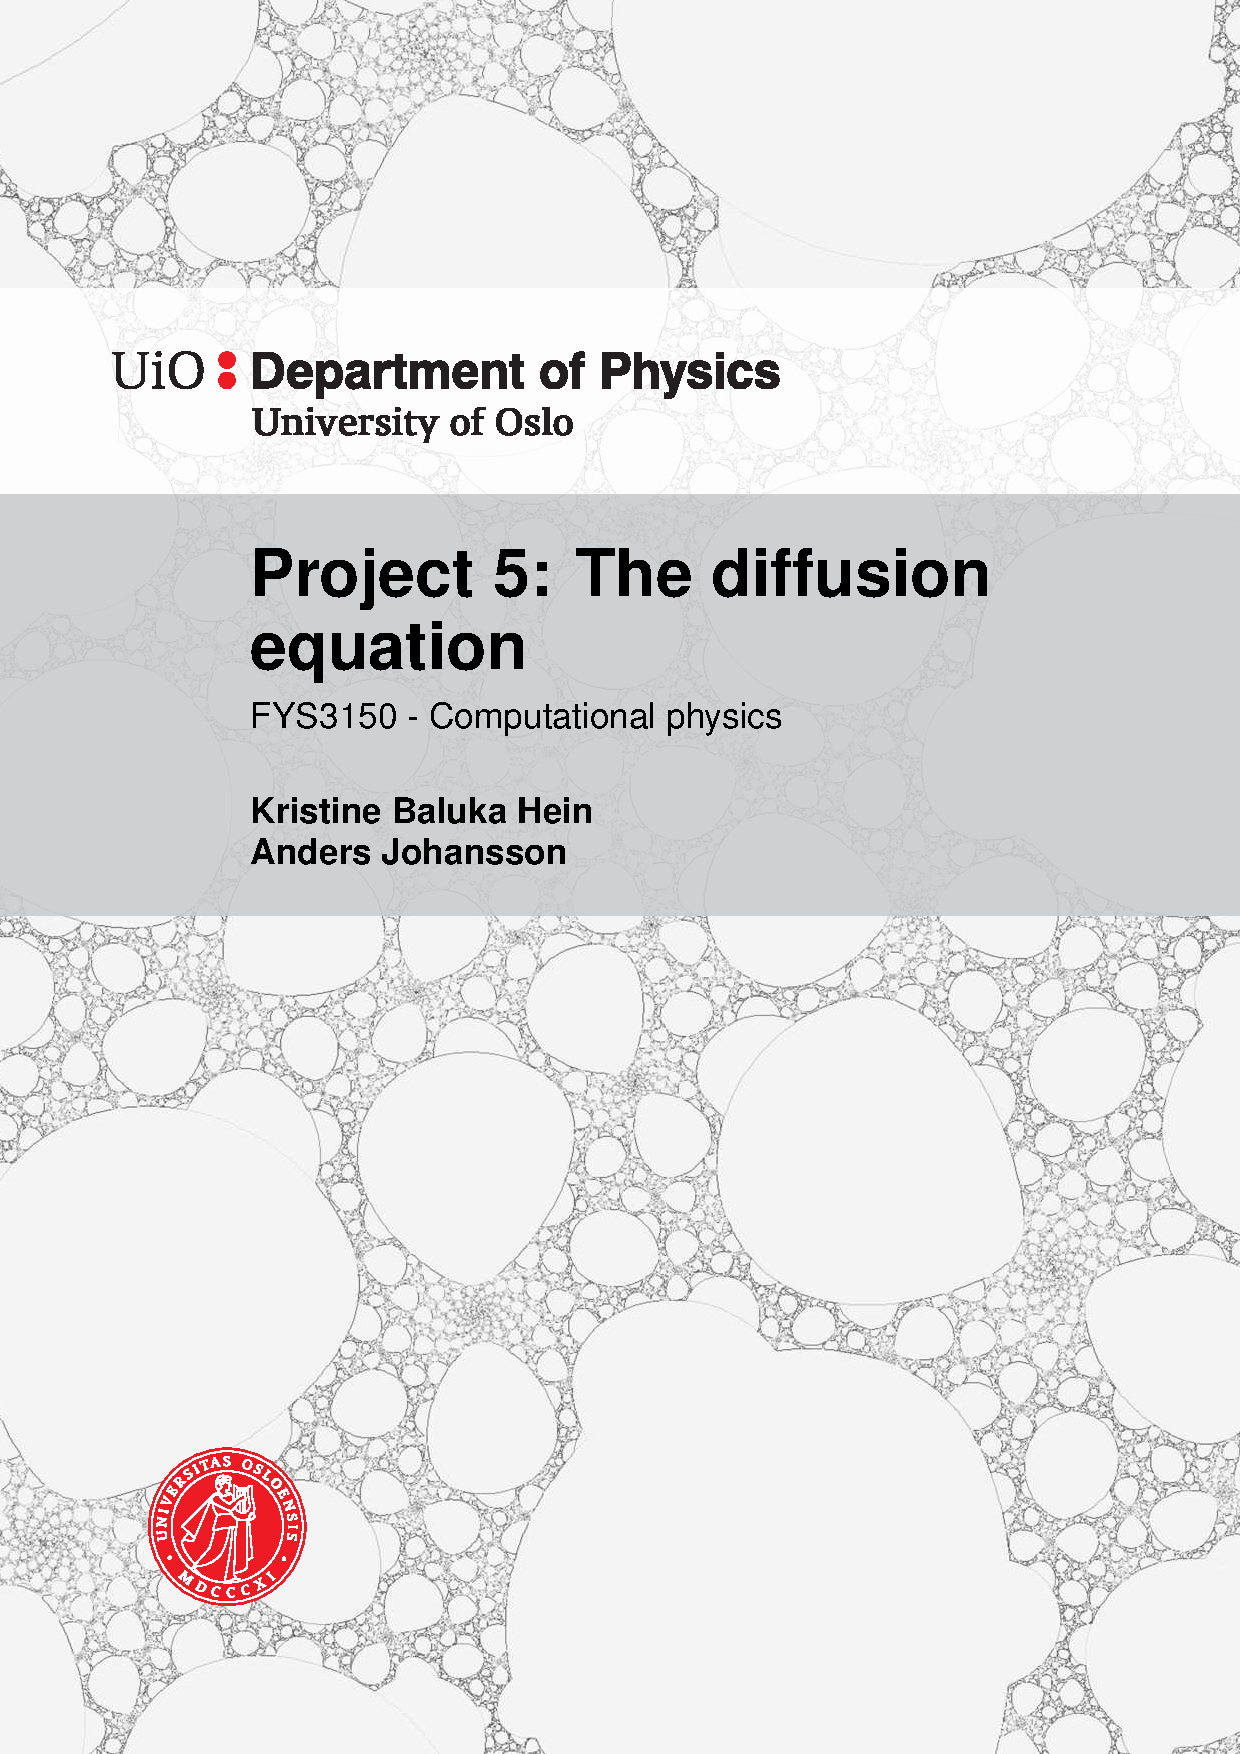
\includepdf{forside.pdf}
%\maketitle
\pagestyle{fancy}
\tableofcontents

\begin{abstract}
In this project, the Ising model for a two-dimensional ferromagnetic is studied numerically using Monte Carlo simulations with the Metropolis algorithm. A \(2\times2\) system is also solved analytically for comparison, and the numerical results fit well. The stability and convergence rate of the Metropolis algorithm are also tested for a \(20\times20\) system. Heavy simulations confirm a phase transition at approximately \(T_C=\num{2.272}\), which is close to the temperature analytically predicted by Lars Onsager.
\end{abstract}
\clearpage


%  _       _                 _            _   _
% (_)_ __ | |_ _ __ ___   __| |_   _  ___| |_(_) ___  _ __
% | | '_ \| __| '__/ _ \ / _` | | | |/ __| __| |/ _ \| '_ \
% | | | | | |_| | | (_) | (_| | |_| | (__| |_| | (_) | | | |
% |_|_| |_|\__|_|  \___/ \__,_|\__,_|\___|\__|_|\___/|_| |_|
\section{Introduction}
The Ising model was developed by the famous physicist Wilhelm Lenz and given to Ernst Ising as a problem for his thesis, in which he found the analytical solution for the one-dimensional situation. Ising's model describes a coupled system in which only the nearest neighbours interact. Aside from describing ferro- and antiferromagnetic materials as in this project, the model has also been used successfully to describe other coupled systems, for instance the development of birdsong dialects\autocite{birdsong}.

In this project, the Ising model is used to describe a two-dimensional ferromagnetic, chrystalline material, modelled as a grid of spins where each spin can have the values \(\pm1\). For an infinite grid, the analytical solution was found by Lars Onsager, while a \(2\times2\) grid is solved analytically in this project.

The problem with analytical solutions for other sizes is finding the partition function, which is the "holy grail" of statistical mechanics. From this quantity, other thermodynamic quantities can be calculated. The difficulty arises from the formula for the partition function, which includes summing over all possible microstates. With each spin having two possible values, a simple \(10\times10\) grid will have \(2^{10\cdot10}\approx10^{30}\) possible microstates. For comparison, only approximately \(10^{17}\) seconds have passed since the creation of the universe. Considering that the UiO computing cluster is capable of approximately \(10^{14}\) calculations per second, it would take this supercomputer at least \(\SI{10}{\percent}\) of the time since Big Bang to calculate the partition function.

As a consequence, calculating the partition function analytically for a grid of reasonable size is not a viable option, and numerical approximations must once again be applied. Fortunately, the Metropolis algorithm, declared one of the top 10 algorithms of the 20th century\autocite{top10algo}, fits the problem very well.

This report starts off with a lenghty introduction, before giving an overview of both the mathematical and the physical theory of the problem at hand. The above mentioned Metropolis algorithm is implemented and tested on the \(2\times2\) grid, for which an analytical solution is also developed. The convergence of the Metropolis algorithm is then tested for a \(20\times20\) grid, and the numerically approximated probability distribution is analysed. Finally, the phase transition is thoroughly studied for varying grid sizes, and the critical temperature is found.

\clearpage
%        _               _           _   _   _
%  _ __ | |__  _   _ ___(_) ___ __ _| | | |_| |__   ___  ___  _ __ _   _
% | '_ \| '_ \| | | / __| |/ __/ _` | | | __| '_ \ / _ \/ _ \| '__| | | |
% | |_) | | | | |_| \__ \ | (_| (_| | | | |_| | | |  __/ (_) | |  | |_| |
% | .__/|_| |_|\__, |___/_|\___\__,_|_|  \__|_| |_|\___|\___/|_|   \__, |
% |_|          |___/                                               |___/
\section{Physical theory}

%  _     _
% (_)___(_)_ __   __ _
% | / __| | '_ \ / _` |
% | \__ \ | | | | (_| |
% |_|___/_|_| |_|\__, |
%                |___/
\subsection{The Ising model}
As stated in the introduction, the Ising model describes a coupled system where nearest neighbours affect each other. In this project, the Ising model is applied to a two-dimensional magnetic material modelled as a grid or lattice of spins, where each spin \(s_i\) can have the values \(+1\) or \(-1\), denoted by \(\uparrow\) and \(\downarrow\) respectively. Assuming that all couplings are of equal magnitude, the coupling in the Ising model leads to the energy
\[
E = -J\sum_{\langle ij\rangle}s_is_j\eqtag{energy}
\]
where the sum is over the nearest neighbours. From this expression, we see that if \(J\) is positive, the energy is minimised when all spins are aligned in parallel, which is the behaviour of a ferromagnetic material. If, on the other hand, \(J\) is negative, a state where all spins are antiparallel to each other has the lowest energy, corresponding to an antiferromagnetic material.

\subsubsection{Borders}
The treatment of the borders of the lattice is a technicality which shows up when the lattice is not infinite. In the so-called thermodynamic limit, where the lattice is infinite, all spins are surrounded the same amount of other spins. With a finite lattice, however, this is not the case, which causes finite size effects.

One possible workaround is to ignore this problem completely, while a smarter alternative is to use what is commonly referred to as periodic boundary conditions. The idea behind this is to simulate an infinite lattice by assuming e.g. that the spins to the right of the right edge of the grid would be equal to the spins on the left edge. This approach has been implemented in \program{ising.cpp}.

%      _        _         _
%  ___| |_ __ _| |_ _ __ | |__  _   _ ___
% / __| __/ _` | __| '_ \| '_ \| | | / __|
% \__ \ || (_| | |_| |_) | | | | |_| \__ \
% |___/\__\__,_|\__| .__/|_| |_|\__, |___/
%                  |_|          |___/
\subsection{Statistical physics}
The basis for the statistical physics of this problem is the probability distribution used for the macrostates, which is the Boltzmann distribution. This distribution states that the probability of a system being in a state with energy \(E_i\) is proportional to \(\exp{-\beta E_i}\), where \(\beta=1/kT\). This probability distribution needs to be normalised, and with the normalisation factor denoted \(1/Z\), we get the equation
\[
1 = \sum_i P(E_i) = \sum_i \frac{1}{Z}\exp{-\beta E_i} = \frac{1}{Z}\sum_i\exp{-\beta E_i} \implies Z = \sum_i \exp{-\beta E_i}
\]
\(Z\) is called the partition function, and is perhaps the most important quantity in statistical physics, as it makes it possible to calculate most other thermodynamic quantities. The energy can be calculated directly as
\[
E = -\pdv{\ln(Z)}{\beta}
\]
In general, the expectation value of any thermodynamic quantity \(A\) can be calculated through
\[
\langle A\rangle = \sum_i A_iP(E_i)
\]
For the two-dimensional Ising model, we are primarily interested in the expectation values of the energy \(E\) and magnetization \(\abs{M}\), as well as the heat capacity \(C_V\) and magnetic susceptibility \(\chi\). The latter quantities can be calculated from the formulas\autocite{compphys}
\begin{alignat*}{2}
C_V &= \frac{1}{kT^2}\qty(\langle E^2\rangle - \langle E\rangle^2)\\
\chi &= \frac{1}{kT}\qty(\langle M^2\rangle - \langle M\rangle^2)
\end{alignat*}

%        _                      _                       _ _   _
%  _ __ | |__   __ _ ___  ___  | |_ _ __ __ _ _ __  ___(_) |_(_) ___  _ __  ___
% | '_ \| '_ \ / _` / __|/ _ \ | __| '__/ _` | '_ \/ __| | __| |/ _ \| '_ \/ __|
% | |_) | | | | (_| \__ \  __/ | |_| | | (_| | | | \__ \ | |_| | (_) | | | \__ \
% | .__/|_| |_|\__,_|___/\___|  \__|_|  \__,_|_| |_|___/_|\__|_|\___/|_| |_|___/
% |_|
\subsection{Phase transitions}
One of the great achievements of the two-dimensional Ising model is its ability to predict a phase transition in ferromagnetic materials, an ability which the one-dimensional version lacks. When a ferromagnetic material is heated, a temperature is reached where the materials suddenly start behaving paramagnetic, i.e. where the magnetic moment drops to zero.

An equally dramatic change, which is easier to analyse numerically, is that both the heat capacity and the magnetic susceptibility diverge when the temperature approaches the critical temperature. As such, the critical temperature can be found numerically as the point where the heat capacity and magnetic susceptibility have their largest value. I have chosen to use the heat capacity, as this settles down more quickly, yielding a smoother function of temperature. One can derive the following expression for the magnetic susceptibility as a function of temperature, which shows the divergence:
\[
\chi(T) \propto \abs{T_C-T}^{-\alpha}
\]
where \(\alpha\) is a positive constant, so \(T=T_C\) leads to a division by zero. The heat capacity has a similar expression.

As the analytical expression for the two dimensional Ising model is known for the thermodynamic limit, it is interesting to attempt an approximation of the critical temperature in the thermodynamic limit based on the values found numerically for finite lattices. To achieve this, we have the relation
\[
T_C(L) - T_C(L=\infty) = aL^{-1/\nu}\eqtag{tcltcinf}
\]
where \(a\) is some unknown constant and \(\nu=1\) can be calculated analytically. To find an expression for \(a\), note that if we subtract the above equations for two values of \(L\) for which \(T_C\) has been calculated numerically, \(T_C(L=\infty)\) cancels and we get
\[
T_C(L_i) - T_C(L_j) = a\qty(L_i^{-1/\nu} - L_j^{-1/\nu}) \implies a = \frac{T_C(L_i)-T_C(L_j)}{L_i^{-1/\nu}-L_j^{-1/\nu}}
\]
The thermodynamic limit can then be calculated using \ref{tcltcinf}:
\[
T_C(L=\infty)=T_C(L_i)-aL_i^{-1/\nu} = T_C(L_i)- \frac{T_C(L_i)-T_C(L_j)}{L_i^{-1/\nu}-L_j^{-1/\nu}}\cdot L_i^{-1/\nu}
\]
for some \(L_i\). Using many, e.g. 4, values \(L_i\) and \(L_j\), we should get a good approximation of the thermodynamic limit. This is calculated in \program{findcritical.py}, where the mean value is calculated.



%                                  _        _   _                   _
%   ___ ___  _ __ ___  _ __  _   _| |_ __ _| |_(_) ___  _ __   __ _| |
%  / __/ _ \| '_ ` _ \| '_ \| | | | __/ _` | __| |/ _ \| '_ \ / _` | |
% | (_| (_) | | | | | | |_) | |_| | || (_| | |_| | (_) | | | | (_| | |
%  \___\___/|_| |_| |_| .__/ \__,_|\__\__,_|\__|_|\___/|_| |_|\__,_|_|
%  _   _              |_|
% | |_| |__   ___  ___  _ __ _   _
% | __| '_ \ / _ \/ _ \| '__| | | |
% | |_| | | |  __/ (_) | |  | |_| |
%  \__|_| |_|\___|\___/|_|   \__, |
%                            |___/
\clearpage
\section{Computational theory}
In this project, the famous Metropolis algorithm is used to do a Monte Carlo simulation of the Ising model. General Monte Carlo methods are based on probabilities and randomness, combined with the law of large numbers, which states that the mean value of a series of experiments will converge towards the expectation value. The Metropolis algorithm is no exception.

As discussed in the introduction, it is not possible to calculate the partition function needed for the Boltzmann distribution. As such, the numerical method has to manage without the partition function. The method used in the Metropolis algorithm chooses to instead look at the ratios of the probabilities, as the partition function will then cancel. Assume that the system is in state \(i\) with energy \(E_i\) and considers jumping to state \(j\) with energy \(E_j\). The ratio of the probabilities of being in these two states then becomes
\[
\frac{P(E_j)}{P(E_i)} = \frac{\exp{-\beta E_j}/Z}{\exp{-\beta E_i}/Z} = \exp{-\beta\qty(E_j-E_i)} = \exp{-\beta\Delta E}
\]
When the energy decreases, \(\Delta E<0\) and the ratio becomes greater than \(1\). When the energy increases, the ratio similarly becomes less than \(1\). The Metropolis algorithm says that if the energy decreases, the proposed change of state should be accepted, otherwise it should be accepted with a probability \(\exp{-\beta\Delta E}\). This balances the attractions towards a state with lower energy and a state with higher multiplicity (entropy), thus minimising Helmholtz's free energy, \(F=E-TS\).

\subsection{The Metropolis algorithm}
Choosing to for each step flip one spin, the above discussion can be summarised as
\begin{enumerate}
\item Choose one of the spins at random.
\item Calculate what the change in energy will be if the spin is flipped.
\item Decide whether to flip the spin or not.
\begin{itemize}
\item If the change in energy is negative: Flip the spin.
\item Else: Draw a random number in the interval \(\qty[0,1]\). Flip the spin if the number is smaller than \(\exp{-\beta\Delta E}\).
\end{itemize}
\item Update expectation values.
\end{enumerate}
With \(L\) rows and \(L\) columns in the lattice, one Monte Carlo cycle denotes the process of \(L^2\) attempts at flipping spins.

\subsection{Technicalities}
While it on paper is straight forward to calculate the energy difference and then \(\exp{-\beta \Delta E}\), calculating an exponential is an expensive computation compared to the flipping of spins. Fortunately, it can be shown\autocite{compphys} that in a two-dimensional lattice, only five different energy differences are possible, namely \(-8J\), \(-4J\), \(0\), \(4J\), \(8J\). As such, the exponentials can be precalculated. In order to calculate the energy difference itself as efficiently as possible, it can also be shown that when flipping spin \(j\),
\[
\Delta E = 2Js_j\sum_{\langle k\rangle} s_k
\]
where \(s_j\) is the spin \emph{before} the flip and the sum is over the nearest neighbours of spin \(j\). Similarly, the change in magnetic moment can be calculated as
\[
\Delta M = -2Js_j
\]
where \(s_j\) again is the spin \emph{before} the flip. Alternatively, the spin can be flipped before the change in magnetic moment is calculated with the opposite sign in the formula above.



%  _                 _                           _        _   _
% (_)_ __ ___  _ __ | | ___ _ __ ___   ___ _ __ | |_ __ _| |_(_) ___  _ __
% | | '_ ` _ \| '_ \| |/ _ \ '_ ` _ \ / _ \ '_ \| __/ _` | __| |/ _ \| '_ \
% | | | | | | | |_) | |  __/ | | | | |  __/ | | | || (_| | |_| | (_) | | | |
% |_|_| |_| |_| .__/|_|\___|_| |_| |_|\___|_| |_|\__\__,_|\__|_|\___/|_| |_|
%             |_|
\clearpage
\section{Implementation}
The Metropolis algorithm discussed above has been implemented fairly straightforwardly in \program{ising.cpp}. \program{phases.cpp} is a utility to run simulations as in \ref{phases}, to which the number of simulations, number of temperatures, etc. can be given as command line arguments. \program{findcritical.py} can then be used to analyse the resulting data file and find the critical temperatures.

To save runtime, certain parts of the programs are run in parallel. The Metropolis algorithm, like most Monte Carlo methods, are generally well suited for parallel programming, as many threads can work on different parts of the problem at the same time, without communicating.

In order to simply do separate parts of the project in parallel, all C++ programs use the \texttt{<thread>} library from the \texttt{C++11} standard. The basic syntax is to create a \texttt{thread} object, where the function to be called and the arguments to the function are given to the constructor, followed by a call to the thread's \texttt{join} method when one wishes to wait for the execution to finish. A simple example from \program{analysis.cpp} is
\lstinputlisting[language=C++,linerange={threadstart-threadend},caption={Example of parallel programming using \texttt{<thread>}.}]{analysis.cpp}
In this snippet, four different Monte Carlo simulations are started as separate threads. Then, the program waits for two of them to finish before starting two other threads which analyse the results from these two. Finally, the program waits for all threads to finish.

I was originally planning to use the \texttt{OpenMPI} library for parallelisation of the phase transition study, but time constraints have forced me to stick with \texttt{<thread>}. As it has not been necessary to split the computations over separate machines, this has not been a problem. It would, however, have enabled the programs to run on several of the computers connected to the HTCondor service at once, which would have been an advantage for the heavy simulations.

The servers at the Department of Informatics as well as their HTCondor service have been used to run the longer simulations in \ref{phases}.

%                      _ _
%  _ __ ___  ___ _   _| | |_ ___
% | '__/ _ \/ __| | | | | __/ __|
% | | |  __/\__ \ |_| | | |_\__ \
% |_|  \___||___/\__,_|_|\__|___/
\clearpage
\section{Results}
All numerical values are given in units of \(J\) and \(k\).

\subsection{Test of parallelisation}
In \program{timetest.cpp}, two Monte Carlo simulations are first run sequentially and then in parallel. If the parallelisation has been successful, the parallel run should take only about half the time of the sequential run, as the two threads can work completely separate of each other.

One technical issue of checking parallelisation is that the normal \texttt{clock} method does not work - this counts CPU cycles, which is the same for the sequential and parallel runs. As the main interest in this test is to get a rough estimate rather than exact runtime, I have chosen to simply use the \texttt{time} and \texttt{difftime} functions, which gives an integer amount of second. The results are
\input{time.dat}
confirming the expected speedup factor of \(2\).

%  ____  _           ____
% |___ \| |__  _   _|___ \
%   __) | '_ \| | | | __) |
%  / __/| |_) | |_| |/ __/
% |_____|_.__/ \__, |_____|
%              |___/
\subsection{Numerical and analytical results for a \(2\times2\) lattice}

%                    _       _   _           _
%   __ _ _ __   __ _| |_   _| |_(_) ___ __ _| |
%  / _` | '_ \ / _` | | | | | __| |/ __/ _` | |
% | (_| | | | | (_| | | |_| | |_| | (_| (_| | |
%  \__,_|_| |_|\__,_|_|\__, |\__|_|\___\__,_|_|
%                      |___/
\subsubsection{Analytical result}
For a \(2\times2\) lattice, the thermodynamic quantities can be found analytically without too much work. To find the partition function, we need to write out all possible microstates and calculate their energies. Using the periodic boundary conditions, we get
\begin{longtable}{ccc}\toprule
Microstate & Energy & Magnetic moment\\ \midrule
\endfirsthead
\midrule
Microstate & Energy & Magnetic moment\\ \midrule
\endhead
\bottomrule
\endlastfoot
    \tilstand{0}{0}{0}{0} & \(E = -8J\) & \(M = -4\)\\ \midrule
    \tilstand{0}{0}{0}{1} & \(E = 0\) & \(M = -2\)\\ \midrule
    \tilstand{0}{0}{1}{0} & \(E = 0\) & \(M = -2\)\\ \midrule
    \tilstand{0}{0}{1}{1} & \(E = 0\) & \(M = 0\)\\ \midrule
    \tilstand{0}{1}{0}{0} & \(E = 0\) & \(M = -2\)\\ \midrule
    \tilstand{0}{1}{0}{1} & \(E = 0\) & \(M = 0\)\\ \midrule
    \tilstand{0}{1}{1}{0} & \(E = 8J\) & \(M = 0\)\\ \midrule
    \tilstand{0}{1}{1}{1} & \(E = 0\) & \(M = 2\)\\ \midrule
    \tilstand{1}{0}{0}{0} & \(E = 0\) & \(M = -2\)\\ \midrule
    \tilstand{1}{0}{0}{1} & \(E = 8J \) & \(M = 0\)\\ \midrule
    \tilstand{1}{0}{1}{0} & \(E = 0 \) & \(M = 0\)\\ \midrule
    \tilstand{1}{0}{1}{1} & \(E = 0 \) & \(M = 2\)\\ \midrule
    \tilstand{1}{1}{0}{0} & \(E = 0 \) & \(M = 0\)\\ \midrule
    \tilstand{1}{1}{0}{1} & \(E = 0 \) & \(M = 2\)\\ \midrule
    \tilstand{1}{1}{1}{0} & \(E = 0 \) & \(M = 2\)\\ \midrule
    \tilstand{1}{1}{1}{1} & \(E = -8J \) & \(M = 4\)\\
\end{longtable}

To summarise, we have
\begin{table}[H]
    \centering
    \begin{tabular}{cccc}\toprule
        Number of \(\uparrow\) & Multiplicity & Energy & Magnetic moment\\ \midrule
        \(4\) & \(1\) & \(-8J\) & \(4\) \\ \midrule
        \(3\) & \(4\) & \(0\) & \(2\) \\ \midrule
        \(2\) & \(2\) & \(8J\) & \(0\) \\ \midrule
        \(2\) & \(4\) & \(0\) & \(0\) \\ \midrule
        \(1\) & \(4\) & \(0\) & \(-2\) \\ \midrule
        \(0\) & \(1\) & \(-8J\) & \(-4\) \\ \bottomrule
    \end{tabular}
\end{table}

Summing over all microstates, we get the partition function
\[
    Z = \sum_{\substack{\text{all}\\ \text{micro-}\\ \text{states}}} \exp{-\beta E_i}
    = 2\exp{8J\beta} + 2\exp{-8J\beta} + 12
\]

The expectation value of the energy can then be found from
\begin{alignat*}{2}
    \langle E\rangle &= -\pdv{\ln(Z)}{\beta} = -\pdv{\beta}(\ln(2\exp{8J\beta} + 2\exp{-8J\beta} + 12))\\
    &= -\frac{1}{2\exp{8J\beta} + 2\exp{-8J\beta} + 12}\qty(16J\exp{8J\beta}-16J\exp{-8J\beta})\\
    &= -\frac{8J\qty(\exp{8J\beta}-\exp{-8J\beta})}{\exp{8J\beta}+\exp{-8J\beta}+6}
\end{alignat*}
yielding the heat capacity
\begin{alignat*}{2}
    C_V &= \pdv{T}(\langle E\rangle) = \pdv{\beta}{T}\pdv{\beta}(\langle E\rangle)=-\frac{1}{kT^2}\pdv{\beta}(\langle E\rangle)\\
    &= -\frac{1}{kT^2}\pdv{\beta}(-\frac{8J\qty(\exp{8J\beta}-\exp{-8J\beta})}{\exp{8J\beta}+\exp{-8J\beta}+6})\\
    &= \frac{8J}{kT^2}\frac{8J\qty(\exp{8J\beta}+\exp{-8J\beta})(\exp{8J\beta}+\exp{-8J\beta}+6)-\qty(\exp{8J\beta}-\exp{-8J\beta})8J\qty(\exp{8J\beta}-\exp{-8J\beta})}{\qty(\exp{8J\beta}+\exp{-8J\beta}+6)^2}\\
    &= \frac{64J^2}{kT^2}\frac{6\qty(\exp{8J\beta}+\exp{-8J\beta})+\qty(\exp{8J\beta}+\exp{-8J\beta})^2-\qty(\exp{8J\beta}-\exp{-8J\beta})^2}{\qty(\exp{8J\beta}+\exp{-8J\beta}+6)^2}\\
    &= \frac{64J^2}{kT^2}\frac{6\qty(\exp{8J\beta}+\exp{-8J\beta})+\exp{16J\beta}+2+\exp{-16J\beta}-\qty(\exp{16J\beta}-2+\exp{-16\beta})}{\qty(\exp{8J\beta}+\exp{-8J\beta}+6)^2}\\
    &= \frac{64J^2}{kT^2}\frac{6\qty(\exp{8J\beta}+\exp{-8J\beta})+4}{\qty(\exp{8J\beta}+\exp{-8J\beta}+6)^2}
\end{alignat*}
To find the various quantities connected to magnetisation, we use the general formula
\[
    \langle A\rangle = \frac{1}{Z}\sum_{\substack{\text{all}\\ \text{micro-}\\ \text{states}}}A_i\exp{-\beta E_i}
\]
Mean magnetic moment(s):
\begin{alignat*}{2}
        \langle M\rangle &= \frac{1}{2\exp{8J\beta} + 2\exp{-8J\beta} + 12}\qty(-4\exp{8J\beta}+4\cdot(-2)+0+0+4\cdot2+4\exp{8J\beta})=0\\
        \langle M^2\rangle &= \frac{1}{2\exp{8J\beta} + 2\exp{-8J\beta} + 12} \qty(\qty(-4)^2\exp{8J\beta}+4\cdot\qty(-2)^2+0+0+4\cdot2^2+4^2\exp{8J\beta})\\
        &= \frac{32\qty(\exp{8J\beta}+1)}{2\exp{8J\beta} + 2\exp{-8J\beta} + 12}
        = \frac{16\qty(\exp{8J\beta}+1)}{\exp{8J\beta} + \exp{-8J\beta} + 6}\\
        \langle \abs{M}\rangle &= \frac{1}{2\exp{8J\beta} + 2\exp{-8J\beta} + 12}\qty(\abs{-4}\exp{8J\beta}+4\cdot\abs{-2}+0+0+4\cdot2+4\exp{8J\beta})\\
        &= \frac{8\qty(\exp{8J\beta}+2)}{2\exp{8J\beta} + 2\exp{-8J\beta} + 12}
        = \frac{4\qty(\exp{8J\beta}+2)}{\exp{8J\beta} + \exp{-8J\beta} + 6}
        \intertext{Magnetic susceptibility:}
        \chi &= \beta\qty(\langle M^2\rangle - \cancel{\langle M\rangle^2})=
    \frac{16\beta\qty(\exp{8J\beta}+1)}{\exp{8J\beta} + \exp{-8J\beta} + 6}
\end{alignat*}

%                                  _           _
%  _ __  _   _ _ __ ___   ___ _ __(_) ___ __ _| |
% | '_ \| | | | '_ ` _ \ / _ \ '__| |/ __/ _` | |
% | | | | |_| | | | | | |  __/ |  | | (_| (_| | |
% |_| |_|\__,_|_| |_| |_|\___|_|  |_|\___\__,_|_|
\subsubsection{Numerical results}
With \(J=1\) and \(\beta=1\), the above expressions give
\begin{alignat*}{8}
\langle E\rangle/L^2 &=& \num{-1.99598} \qquad&& C_V/L^2 &=& \num{0.03208}\\
\langle \abs{M}\rangle/L^2 &=& \num{0.99866} \qquad&& \chi/L^2 &=& \num{3.9933}
\end{alignat*}

Running \(\num{100000}\) Monte Carlo cycles with the same parameters gives \vref{2by2}.

\begin{figure}[H]
\centering
\input{2by2.plt}\caption{Numerical results from \num{100000} Monte Carlo cycles. Generated by \program{2by2.cpp}.}\label{2by2}
\end{figure}

These results fit fairly well with the numbers calculated above, but we see from the graphs that the values for the heat capacity and magnetic susceptibility have yet to settle down completely. Running \(\num{10000000}\) Monte Carlo cycles yields
\input{2by2res.dat}
These results fit very well with the analytical results.


%                    _           _
%   __ _ _ __   __ _| |_   _ ___(_)___
%  / _` | '_ \ / _` | | | | / __| / __|
% | (_| | | | | (_| | | |_| \__ \ \__ \
%  \__,_|_| |_|\__,_|_|\__, |___/_|___/
%                      |___/
\subsection{Analysis}
\begin{figure}[H]
\centering
\input{randomanalysis.plt}\caption{Simulation for \(10^6\) Monte Carlo cycles with two different temperatures and random initial states. Generated by \program{analysis.cpp}.}\label{2020random}
\end{figure}
\begin{figure}[H]
\centering
\input{orderedanalysis.plt}\caption{Simulation for \(10^6\) Monte Carlo cycles with two different temperatures and all spins initially pointed upwards. Generated by \program{analysis.cpp}.}\label{2020ordered}
\end{figure}
Comparing \ref{2020random} and \ref{2020ordered}, we see that the initial state has very little to say for the final values, as well as the time it takes to reach a steady state\footnote{Note that the \(y\)-axis is logarithmic in the plots for heat capacity and magnetic susceptibility, thus greatly exaggerating the difference in choice of initial state.}.

\subsubsection{Number of accepted flips}
\begin{figure}[H]
\centering
\input{accepted.plt}
\caption{The number of accepted flips as a function of the number of Monte Carlo cycles, on a logarithmic scale. Generated by \program{analysis.cpp} and \program{accepted.gpi}.}\label{fig:accepted}
\end{figure}
As the number of accepted flips should grow linearly as a function of the number of Monte Carlo cycles when the system is in equilibrium, we see that \(\num{10000}\) cycles seems sufficient to reach a steady state, as the graphs are approximately linear with a derivative of 1 from this point.

\subsubsection{Numerical probability distribution}
\begin{figure}[H]
\centering
\input{probdist.plt}
\caption{Counting the ocurrences of the different energy levels. For practical reasons, the counting includes all Monte Carlo cycles. This has negligible effect on the resulting histograms. Generated by \program{analysis.cpp} and \program{probdist.gpi}.}
\end{figure}
When the temperature is higher, it is expected that the mean energy is higher, and also that the energy distribution is more spread out and more states are visited. This fits very well with the histograms above. The number of visited energy levels also fits with \vref{fig:accepted}, where the number of accepted changes of state is much higher when the temperature is higher, giving a larger variance and heat capacity, as seen in \vref{2020random}.


%        _                      _                       _ _   _
%  _ __ | |__   __ _ ___  ___  | |_ _ __ __ _ _ __  ___(_) |_(_) ___  _ __  ___
% | '_ \| '_ \ / _` / __|/ _ \ | __| '__/ _` | '_ \/ __| | __| |/ _ \| '_ \/ __|
% | |_) | | | | (_| \__ \  __/ | |_| | | (_| | | | \__ \ | |_| | (_) | | | \__ \
% | .__/|_| |_|\__,_|___/\___|  \__|_|  \__,_|_| |_|___/_|\__|_|\___/|_| |_|___/
% |_|
\subsection{Discovering a phase transition}\label{phases}

\begin{figure}[H]
\centering
\input{40atcondor.plt}
\caption{Simulation for 40 different temperatures with \(\num{100000}\) Monte Carlo cycles (after skipping \(\num{20000}\)). Run by \program{condorquick.cmd} on the HTCondor system and generated by \program{phases.cpp}.}
\end{figure}
From the figure, we see that the heat capacity magnetic susceptibility peak at a temperature around \(\num{2.3}\). Unfortunately, it is clear that more data is required in order to get reasonable results.

The above graph of the susceptibility gives the following maxima for the heat capacity, ideally corresponding to the critical temperatures:
\input{40atcondor.dat}
This was calculated by \program{findcritical.py}.

\begin{figure}[H]
\centering
\input{40atcondorlong.plt}
\caption{Simulation for 40 different temperatures with \(\num{500000}\) Monte Carlo cycles (after skipping \(\num{20000}\)). Run by \program{condormedium.cmd} on the HTCondor system and generated by \program{phases.cpp}. The runtime was approximately 4 hours.}\label{5e5}
\end{figure}
With five times as many Monte Carlo cycles, the data look a bit better and have a lot less noise, while still not super.

The above graph of the susceptibility gives the following maxima for the heat capacity, ideally corresponding to the critical temperatures:
\input{40atcondorlong.dat}
This was calculated by \program{findcritical.py}. This is very close to Lars Onsager's analytical result of \(T_C(L=\infty)=\num{2.269}\). With 40 temperatures in the interval from \(\num{2.2}\) to \(\num{2.4}\), this is nearing the maximum precision possible.


\begin{figure}[H]
\centering
\input{40with2E6.plt}
\caption{Simulation for 40 different temperatures with \(\num{2E6}\) Monte Carlo cycles (after skipping \(\num{20000}\)). Run on a UiO server (with 64 cores) and generated by \program{phases.cpp}. The runtime was approximately 15.5 hours.}\label{2e6}
\end{figure}
With this many Monte Carlo cycles and a ginormous runtime, I was hoping for the graph of the magnetic susceptibility to look considerably better. The heat capacity, on the other hand, has improved, and this is the quantity used to calculate the critical temperature.
\input{40with2E6.dat}
This was calculated by \program{findcritical.py}. While the graphs don't look particularly pretty, the approximation to the thermodynamic limit is even closer to Lars Onsager's analytical result of \(T_C(L=\infty)=\num{2.269}\), and the distance is approximately equal to the best achievable accuracy with this choice of temperatures.

Unfortunately, the values for the expectations values for the energy and magnetisation in \ref{5e5} and \ref{2e6} are quite clearly wrong, which probably stems from these runs not being done with the latest versions of the programs due to the runtime (the simulation generating the data in \ref{2e6} finished just two hours before the deadline). The critical temperatures are, however, not affected by this. I believe the error was caused by how the "skip the first steps" ability was implemented, as the implementation was changed without certain lines being updated, leading to a division by the wrong amount of Monte Carlo cycles. I may eventually redo these runs and upload the updated report on GitHub.


%                       _           _
%   ___ ___  _ __   ___| |_   _ ___(_) ___  _ __
%  / __/ _ \| '_ \ / __| | | | / __| |/ _ \| '_ \
% | (_| (_) | | | | (__| | |_| \__ \ | (_) | | | |
%  \___\___/|_| |_|\___|_|\__,_|___/_|\___/|_| |_|
\clearpage
\section{Conclusion}
In this project, the magnetic properties of a ferromagnetic material has been studied through the Ising model. We started off with the comparison of numerical and analytical results for a \(2\times2\) lattice, where it was shown that the results from the numerical simulations are indeed satisfactory. Then, the behaviour of the system over the course of the simulation was studied for two different temperatures, including the path towards a steady state. Finally, the various thermodynamic quantities were studied as functions of temperature using data from heavy simulations, and a critical temperature was found - both for the finite systems studied numerically and for the thermodynamic limit of an infite lattice. The results agree with the analytical result \(T_C=\num{2.269}\) found by Lars Onsager.

The main idea for further work is to do heavier simulations of the phase transitions, in order to get a smoother function of temperature with less noise, and thus a more precise value for the critical temperature in the thermodynamic limit. I did unforunately not have time to do this. This probably requires the change from \texttt{<thread>} to \texttt{OpenMPI} as a mean for parallelisation, as \texttt{OpenMPI} is a message parsing interface, enabling the programs to be run on multiple machines. On HTCondor, this would allow the program to run on many desktop machines at once.


\clearpage
\addcontentsline{toc}{section}{References}
\printbibliography


\end{document}
